\documentclass[tikz,border=5]{standalone}
\usepackage{amsmath,amssymb,bm}
\usetikzlibrary{arrows.meta,calc,positioning}
\begin{document}

% Original author: Izaak Neutelings (November 2020)
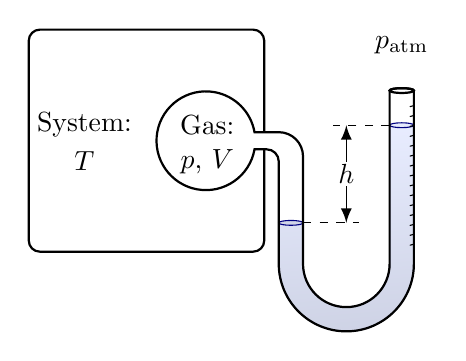
\begin{tikzpicture}
\usetikzlibrary{patterns,decorations.pathmorphing}
\colorlet{mydarkblue}{blue!50!black}
\colorlet{myred}{red!65!black}
\colorlet{watercol}{blue!80!cyan!10!white}
\colorlet{darkwatercol}{blue!80!cyan!20!white}
\tikzstyle{piston}=[blue!50!black,top color=blue!30,bottom color=blue!50,middle color=blue!20,shading angle=0]
\tikzstyle{water}=[draw=mydarkblue,top color=watercol!90,bottom color=watercol!90!black,shading angle=5]
\tikzstyle{vertical water}=[water,
  top color=watercol!90!black!90,bottom color=watercol!90!black!90,middle color=watercol!80,shading angle=90]
\def\tick#1#2{\draw[thick] (#1)++(#2:0.1) --++ (#2-180:0.2)}

  \def\W{1.2}       % pressure box width
  \def\H{1.2}       % pressure box height
  \def\Rx{0.55}     % tube bend radius horizontal
  \def\Ry{0.2*\Rx}  % tube bend radius vertical
  \def\rx{0.28*\Rx} % tube radius horizontal
  \def\ry{0.28*\Ry} % tube radius vertical
  \def\HL{1.3}      % tube height left
  \def\HR{2.2}      % stube height right
  \def\hL{0.40*\HL} % water level height left
  \def\hR{0.80*\HR} % water level height right
  %\def\th{2.7*\H}   % tube height
  %\def\ty{0.93*\th} % tube level
  \def\N{14}
  \draw[water]
    (-\Rx,\hL) --++ (0,-\hL) arc(180:360:\Rx) --++ (0,\hR) --++ (2*\rx,0) --++
    (0,-\hR) arc(360:180:\Rx+2*\rx) --++ (0,\hL);
  \draw[water]
    (-\Rx-\rx,\hL) ellipse({\rx} and {\ry})
    (\Rx+\rx,\hR) ellipse({\rx} and {\ry});
  % \draw[thick]
  %   (-\Rx,\HL) --++ (0,-\HL) arc(180:360:\Rx) --++ (0,\HR) arc(180:0:{\rx} and \ry)
  %   --++ (0,-\HR) arc(360:180:\Rx+2*\rx) --++ (0,\HL)
  %   arc(0:90:\rx) --++ (-\rx,0) --++ (0,0.7*\rx-\H/2) -|++ (-\W,\H) -|++ (\W,0.7*\rx-\H/2)
  %   --++ (2*\rx,0) arc(90:0:2*\rx) -- cycle;
  \draw[thick]
    (-\Rx,\HL) --++ (0,-\HL) arc(180:360:\Rx) --++ (0,\HR) arc(180:0:{\rx} and \ry)
    --++ (0,-\HR) arc(360:180:\Rx+2*\rx) --++ (0,\HL)
    arc(0:90:\rx) --++ (-\rx,0) arc(350:10:1.14*\Rx)--++ (2*\rx,0) arc(90:0:2*\rx) -- cycle;
  \draw[thick]
    (\Rx+\rx,\HR) ellipse({\rx} and \ry);
  \foreach \i [evaluate={\y=(\hL+\hR)/2+0.8*\HR*(\i-\N/2)/\N;}] in {0,...,\N}{
    \draw[line cap=round] (\Rx+2*\rx+0.007,\y) arc(0:-50:{\rx} and \ry);
  }
  %\draw[line cap=round,myred] (\Rx+2*\rx+0.007,{(\hL+\hR)/2}) arc(0:-180:{\rx} and \ry);
  %\draw[line cap=round,myred] (-\Rx+0.007,{(\hL+\hR)/2}) arc(0:-180:{\rx} and \ry);
  \node at (-\W/2-4*\rx-\Rx,\HL+3*\rx) {Gas:};
  \node at (-\W/2-4*\rx-\Rx,\HL+0*\rx) {$p$, $V$};
  \node[above=0.3] at (\Rx+\rx,\HR+\ry) {$p_\mathrm{atm}$};
  
  \node[centered] at (-\Rx-4*\rx-1.8*\W,\HL+3*\rx) {System:};
  \node[centered] at (-\Rx-4*\rx-1.8*\W,\HL+0*\rx) {$T$};

  \draw[thick,rounded corners] (-\Rx-3.2*\rx,\HL+\rx)--++(0,-\HL)--++(-2.3*\HL,0)--++(0,2*\HL+2*\Ry)--++(2.3*\HL,0)--++(0,-\HL);

  %\draw[thick,red] (-\Rx-3.5*\rx,\HL+\rx)--++(0,2*\Ry);
  
  \draw[dashed] (-\Rx,\hL) --++ (1.3*\Rx,0) (\Rx,\hR) --++ (-1.3*\Rx,0);
  \draw[latex-latex] (0,\hL) -- (0,\hR) node[midway,fill=white,inner sep=1] {$h$};
\end{tikzpicture}

\end{document}
